\paragraph{Ridge Regression}
\subparagraph{Definition}
\sB{The ridge regression coefficient estimates $\hat{\beta}^{R}$ are 
the values that minimize}:
\begin{center}
\encV{$
\su{{i=1}}{n}\left( y_{i}-\beta_{0}-\su{{j=1}}{p}\beta_{j}x_{ij} \right)^{2} + \lambda\su{{j=1}}{p}\beta_{j}^{2}=RSS+\lambda\su{{j=1}}{p}\beta_{j}^{2}
$}
\end{center}
where $\lambda > 0$ is a \emph{turning parameter} to be determined 
separately.\\
$RSS(\lambda)=(\bm{y}-\bm{X}\beta)^{T}(y-\bm{X}\beta)+\lambda\beta^{T}\beta$\\
\begin{center}
	\enc{$\hat{\beta}^{ridge}=(\bm{X}^{T}\bm{X}+\lambda\bm{I})^{-1}\bm{X}^{T}\bm{y}$}
\end{center}
In the case of orthonormal inputs, the ridge estimates are just a
scaled version of the least squares estimates, that is 
\tB{$\hat{\beta}^{ridge}=\frac{1}{1+\lambda}\hat{\beta}$}\\
The \tR{Singular Value Decomposition (SVD)} of the centered input matrix
$\bm{X}$ gives us some additional insight into the nature of ridge 
regression:
The $SVD$ of the $N\times p$ matrix $\bm{X}$ has the form:
\begin{center}
	\encB{$\bm{X} = \bm{UD}\bm{V}^{T}$}
\end{center}
Here \sB{$\bm{U}$ and $\bm{V}$ are $N\times p$ and $p\times p$ orthogonal
matrices}, with the columns of \sB{$\bm{U}$ spanning the columns space} of
$\bm{X}$, and the columns of \sB{$\bm{V}$ spanning the row space}.\\
$\bm{D}$ is a $p\times p$ diagonal matrix, containing singular values
of $\bm{X}$
Using the singular value decomposition:
\begin{align*}
	\bm{X}\hat{\beta}^{ls} &= \bm{X}(\bm{X}^{T}\bm{X})^{-1}\bm{X}^{T}\bm{y}\\
	&= \bm{U}\bm{U}^{T}\bm{y}
\end{align*}
For ridge regression:
\begin{align*}
	\bm{X}\hat{\beta}^{ridge} &= \bm{X}(\bm{X}^{T}\bm{X}+\lambda\bm{I})^{-1}\bm{X}^{T}\bm{y}\\
	&= \bm{U}\bm{D}(\bm{D}^{2}+\lambda\bm{I})^{-1}\bm{D}\bm{U}^{T}\bm{y}\\
	&= \su{{j=1}}{p}u_{j}\dfrac{d_{j}^{2}}{d_{j}^{2}+\lambda}u_{j}^{T}\bm{y}
\end{align*}
Like linear regression, \sB{ridge regression computes the coordinates of 
$\bm{y}$ with respect to the orthonormal basis $\bm{U}$, It shrinks
these coordinates by} \tB{$\dfrac{d_{j}^{2}}{d_{j}^{2}+\lambda}$}, a greater
amount of shrinkage is applied to the coordinates of basis vectors with
smaller $d_{j}^{2}$\\
The SVD of the centered matrix $X$ is another way to express the 
principal components of the variables in $\bm{X}$. The sample 
covariance matrix is given by $\bm{S}=\dfrac{\bm{X}^{T}\bm{X}}{N}$
\begin{center}
	$\bm{X}\bm{X}^{T}=\bm{V}\bm{D}^{2}\bm{V}^{T}$
\end{center}
which is the eigen decomposition of $\bm{X}^{T}\bm{X}$\\
The eigenvectors $v_{j}$ are also called the principal components 
directions of $\bm{X}$. The first principal component direction 
$v_{1}$ has the property that $z_{1}=\bm{X}v_{1}$ has the largest
sample variance amongst all normalized linear combinations of the 
columns of $\bm{X}$:
\begin{center}
	$\V{z_{1}}=\V{\bm{X}v_{1}}=\dfrac{d_{1}^{2}}{N}$
\end{center}
\begin{figure}[H]
	\begin{center}
		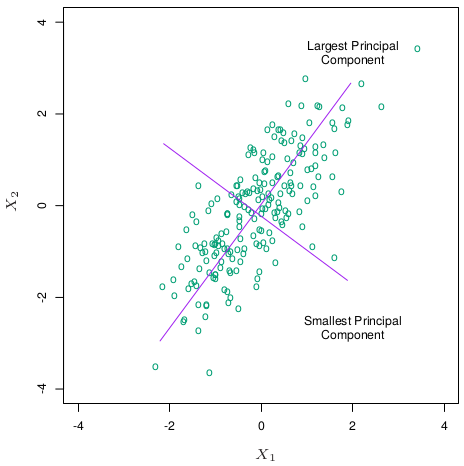
\includegraphics[width=.5\textwidth]{./chap/1chap/5sec/images/4_PrincipalComponentsRidge.png}
	\end{center}
	\caption{The largest principal components is the direction that
	maximizes the variance of the projected data and the smallest
	principal component minimizes that variance.
	\tB{Ridge regression projects $\bm{y}$ onto these components, and 
	then shrinks the coefficients of the low-variance components 
	more than the high-variance components}}
	\label{fig:5.4_PrincipalComponentsRidge}
\end{figure}
\begin{align*}
	df(\lambda) &=tr\left(\bm{X}(\bm{X}^{T}\bm{X}+\lambda\bm{I})^{-1}\bm{X}^{T}\right)\\
	&= tr(\bm{H}_{\lambda})\\
	&= \su{{j=1}}{p}\dfrac{d_{j}^{2}}{d_{j}^{2}+\lambda}
\end{align*}
This monotone decreasing function of $\lambda$ is the \emph{effective
degrees of freedom} of the ridge regression fit.\\
Note that \tB{$df(\lambda)=p$ when $\lambda=0$ (no regularization) and
$df(\lambda)\rightarrow 0$ as $\lambda\rightarrow \infty$}

\subparagraph{Why does Ridge Regression improve over Least Squares?}
Ridge regression's advantage over least squares is rooted in the 
\emph{bias-variance trade-off}. \tR{As $\lambda$ increases, the 
flexibility of the ridge regression fit decreases, leading to decreased
variance but increased bias.}

\begin{python}
reg = linear_model.Ridge(alpha=0.5)
reg.fit([[0, 0], [0, 0], [1, 1]], [0, 1, 1])
print(reg.coef_)
\end{python}
\paragraph{The Lasso}
It is a relatively recent alternative to ridge regression.\\
\sB{The Lasso coefficients, $\hat{\beta}_{\lambda}$ minimize the
quantity}:
\begin{center}
\encV{
$
\su{{i=1}}{n}\left( y_{i}-\beta_{0}-\su{{j=1}}{p}\beta_{j}x_{ij} \right)^{2}+\lambda\su{{j=1}}{p}|\beta_{j}| = RSS +\lambda\su{{j=1}}{p}|\beta_{j}|
$}
\end{center}
\tB{Models generated from the lasso are generally much easier to 
interpret than those produced by ridge regression.}
\begin{python}
reg = linear_model.Lasso(alpha=0.1)
reg.fit([[0, 0], [1, 1]], [0, 1])
print(reg.coef_)
\end{python}

\subparagraph{Another formulation for Ridge Regression and the Lasso}
\begin{center}
\encV{
$
\begin{cases}
	\min\limits_{\prtH{\beta}{j}{0}{p}}\left\{ \su{{i=1}}{n}\left( y_{i-}-\beta_{0}-\su{{j=1}}{p}\beta_{j}x_{ij} \right)^{2} \right\}\text{ subject to }\su{{j=1}}{p}|\beta_{j}|\leq s\text{ Ridge Regression}\\
	\min\limits_{\prtH{\beta}{j}{0}{p}}\left\{ \su{{i=1}}{n}\left( y_{i-}-\beta_{0}-\su{{j=1}}{p}\beta_{j}x_{ij} \right)^{2} \right\}\text{ subject to }\su{{j=1}}{p}\beta_{j}^{2}\leq s\text{ Lasso}
\end{cases}
$}
\end{center}

\paragraph{The variable selection property of the Lasso}
The least squares solution is marked as $\hat{\beta}$.
\begin{figure}[H]
	\begin{center}
		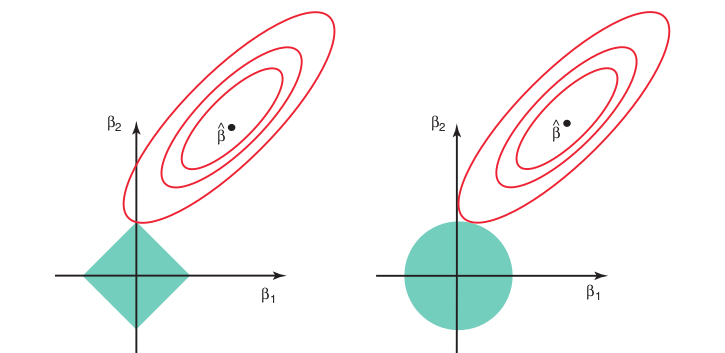
\includegraphics[width=\textwidth]{./chap/1chap/5sec/images/1RSSelipses.png}
	\end{center}
	\caption{Contours of the error and constraint functions for the
	lasso (left) and ridge regression (right). The solid blue areas
	are the constraint regressions, $|\beta_{1}|+|\beta_{2}|\leq 
	s\text{ and }\beta_{1}^{2}+\beta_{2}^{2}\leq s$, while the red
	ellipses are the contours of the RSS (all of the points on a
	given ellipse share a common value of the RSS).}
	\label{fig:5.1 RSSelipses}
\end{figure}

\sB{Since ridge regression has a circular contraint with no sharp
points, this intersection will not generally occur on an axis, and so
the
ridge regression coefficient estimates will be exclusively non-zero.}\\
However, the lasso constraint has \emph{corners} at each of the axes, 
and so the ellipse will often intersect the constraint region at an 
axis.

\subparagraph{Comparing the Lasso and Ridge Regression}
In general, one might expect \tB{the lasso to perform better in a
setting where a relatively small number of predictors have a 
substantial coefficients}, and the remaining predictors have 
coefficients that are very small or that equal zero.\\
\tB{Ridge regression will perform better when the response is a
function of many predictors}, all with coefficients of roughly equal 
size.\\

\tR{A technique such as cross-validation can be used in order to
determine which approach is better on a particular data set.}

\subparagraph{Bayesian Interpretation}
\tB{It assumes that the coefficient vector $\beta$ has some \emph{
prior} distribution}, say $p(\beta)$, where $\beta=
\begin{pmatrix}
	\beta_{0}\\
	.\\
	.\\
	.\\
	\beta_{p}
\end{pmatrix}
$
The likelihood of the data can be written as $f(Y|X,\beta)$, where
$X=
\begin{pmatrix}
	X_{1}\\
	.\\
	.\\
	.\\
	X_{p}
\end{pmatrix}
$
\sB{Multiplying the prior distribution by the likelihood gives us (up to a
proportionality constant) the posterior distribution} which takes the
form:\\
$
p(\beta|X,Y)\propto f(Y|X,\beta)p(\beta|X)=f(Y|X,\beta)p(\beta)
$\\
We assume that $Y=\beta_{0}+\su{{i=1}}{p}X_{i}\beta_{i}+\epsilon$ and:
$p(\beta)=\prd{{j=1}}{p}g(\beta_{j})$, for some density function $g$.\\
$g\hookrightarrow\mathcal{N}(0,f(\lambda)^{2})\Rightarrow$ the most
likely value for $\beta$ is given by the \emph{Ridge Regression} 
solution\\
$g\hookrightarrow Laplace(0,f(\lambda))\Rightarrow$ the posterior mode
for $\beta$ is the \emph{Lasso Regression} solution.
\begin{figure}[H]
	\begin{center}
		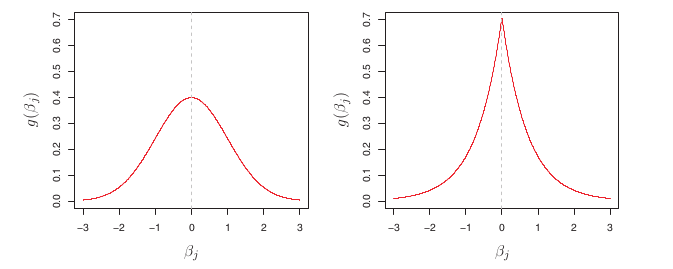
\includegraphics[width=\textwidth]{./chap/1chap/5sec/images/2bayesianPointOfView.png}
	\end{center}
	\caption{Left: Ridge regression is the posterior mode for 
	$\beta$ under a Gaussian prior.\\
	Right: The lasso is the posterior mode for $\beta$ under a 
	double-exponential prior.}
	\label{fig:2bayesianPointOfView}
\end{figure}
We can generalize ridge regression and the lasso, and view them as 
Bayes estimates:
\begin{center}
	\enc{
	$\tilde{\beta}=\min\limits_{\beta}\left\{
	\su{{i=1}}{N}\left(y_{i}-\beta_{0}-
	\su{{j=1}}{p}x_{ij}\beta_{j}\right)^{2}+
	\lambda\su{{j=1}}{p}|\beta_{j}|^{q}\right\}$}
\end{center}
for $q\geq 0$
The value:
$
\begin{cases}
	q=0:\text{ \emph{subset selection} the penalty
	counts the number of nonzero parameters}\\
	q=1:\text{ the \emph{lasso}}\\
	q=2:\text{ the \emph{ridge regression}}
\end{cases}
$\\
The case $q=1$ (lasso) is the smallest $q$ such that the constraint
region is convex: \sV{non-convex constraint regions make the optimization
problem more difficult}.
\begin{figure}[H]
	\begin{center}
		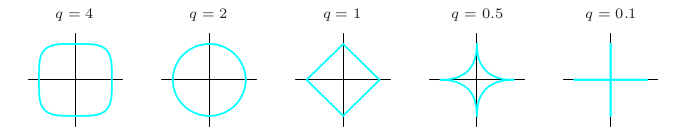
\includegraphics[width=.7\textwidth]{./chap/1chap/5sec/images/5_penaltyContours.png}
	\end{center}
	\caption{Contours of constant value of 
	$\su{j}{}|\beta_{j}|^{q}$}
	\label{fig:5.5_penaltyContours}
\end{figure}
\paragraph{Elastic-net}
\begin{center}
	\enc{$\lambda\su{{j=1}}{p}\left(\alpha\beta_{j}^{2}+(1-\alpha)|\beta_{j}|\right)$}
\end{center}
\begin{python}
reg = linear_model.ElasticNet(random_state=0)
reg.fit([[0, 0], [1, 1]], [0, 1])
print(reg.coef_)
\end{python}

\paragraph{Selecting the Tuning Parameter}
Cross-validation provides a simple way to select $\lambda$ or 
equivalently $s$:\\
\begin{itemize}
	\item We choose a grid of $\lambda$ values
	\item We compute the cross-validation for each value of 
		$\lambda$
	\item We select the tuning parameter value for which the 
		cross-validation error is smallest.
\end{itemize}
Finally the model is re-fit using all of the available observations and
the selected value of the tuning parameter.
\begin{python}
X, y = load_diabetes(return_X_y=True)
clf = RidgeCV(cv = 5, random_state=0).fit(X, y)
print(clf.alpha_)

clf = LassoCV(cv = 5, random_state=0).fit(X, y)
print(clf.alpha_)

clf = ElaticNet(cv = 5, random_state=0).fit(X, y)
print(clf.alpha_) # corresponds to lambda
print(clf.l1_ratio_) # corresponds to alpha
\end{python}

\paragraph{Least Angle Regression}
\subparagraph{Least Angle Regression}
\begin{enumerate}
	\item \sB{Standardize the predictors} to have mean zero an unit 
		norm.\\ \sB{Start with the residual $\bm{r}=\bm{y}-
		\overline{\bm{y}}$}, and for all $i\in\inter{1}{p}
		\beta_{i}=0$
	\item Find the predictor $x_{j}$ most correlated with $\bm{r}$
	\item Move $\beta_{j}$ from 0 to its least-squares coefficient
		$\dfrac{\sP{\bm{x}_{j}}{\bm{r}}}{\sP{\bm{x}_{j}}{\bm{x}_{j}}}$, then recompute 
		$\bm{r}$. Find the predictor $x_{k}$ most correlated with the new $\bm{r}$
	\item Move $\beta_{k}$ from 0 to its least-squares coefficient
		$\dfrac{\sP{\bm{x}_{k}}{\bm{r}}}{\sP{\bm{x}_{k}}{\bm{x}_{k}}}$, then recompute 
		$\bm{r}$. Find the predictor $x_{l}$ most correlated with the new $\bm{r}$\dots
%	\item Move $\beta_{j}$ and $\beta_{k}$ in the direction defined
%		by their joint least squares coefficient of the current
%		residual on $(x_{j},x_{k})$, until some other 
%		competitor $x_{l}$ has as much correlation with the
%		current residual.
	\item Continue in this way until all $p$ predictors have been
		entered. After $\min(N-1, p)$ steps, we arrive at the
		full least-squares solution.
\end{enumerate}
Suppose $\mathcal{A}_{k}$ is the active set of variables at the 
beginning of the $k^{th}$ step and let $\beta_{\mathcal{A}_{k}}$ be the
coefficient vector for these variables at this step, there will be 
$k-1$ nonzero values and the one just entered will be zero.\\
If \sB{$\bm{r}_{k}=\bm{y}-\bm{X}_{\mathcal{A}_{k}}\beta_{\mathcal{A}_{k}}$}
is the current residual, then the direction for this step is:
\begin{center}
	$\delta_{k}=(\bm{X}_{\mathcal{A}_{k}^{T}}\bm{X}_{\mathcal{A}_{k}^{T}})^{-1}\bm{X}_{\mathcal{A}_{k}^{T}}^{T}\bm{r}_{k}$
\end{center}
The name ``least angle'' arises from a geometrical interpretation of 
this process; $\bm{u}_{k}$ makes the smallest (and equal) angle with
each of the predictors in $\mathcal{A}_{k}$
Advantages and Disadvantages:
\begin{itemize}
	\item[\tV{+}] Numerically efficient when $p\gg n$
	\item[\tV{+}] As fast as forward selection and has the same order of complexity as OLS
	\item[\tV{+}] Produces a full piecewise linear solution path
	\item[\tV{+}] Stable
	\item[\tV{+}] Esealy modified to produce for other estimators like the Lasso
	\item[\tR{-}] Because LARS is based upon iterative refitting of the residuals, it would
		appears to be especially sensitive to the effect noise.
\end{itemize}

\subparagraph{Least Angle Regression: Lasso Modification}
\begin{itemize}
	\item[4a] If a non-zero coefficient hits zero, drop its variable from the
		active set of varibalbes and recompute the current joint least squares
		direction
\end{itemize}
\begin{python}
reg = Lars()
reg.fit([[ -1, 1], [0, 0], [1, 1]], [-1.1111, 0, -1.1111])
print(reg.coef_)
\end{python}
